\hspace{-0.1in}
\tikzstyle{input_neuron}=[circle,draw=red!50,fill=red!10,thick,minimum size=8mm]
\tikzstyle{hidden_neuron}=[circle,draw=blue!50,fill=cyan!10,thick,minimum size=8mm]
\tikzstyle{output_neuron}=[circle,draw=green!50,fill=green!10,thick,minimum size=8mm]
\tikzstyle{bias_neuron}=[circle,draw=red!50,fill=red!10,thick,minimum size=4mm]
\tikzstyle{bias_hidden_neuron}=[circle,draw=blue!50,fill=cyan!10,thick,minimum size=4mm]

\tikzstyle{input}=[circle,draw=black!50,fill=black!20,thick,minimum size=8mm]

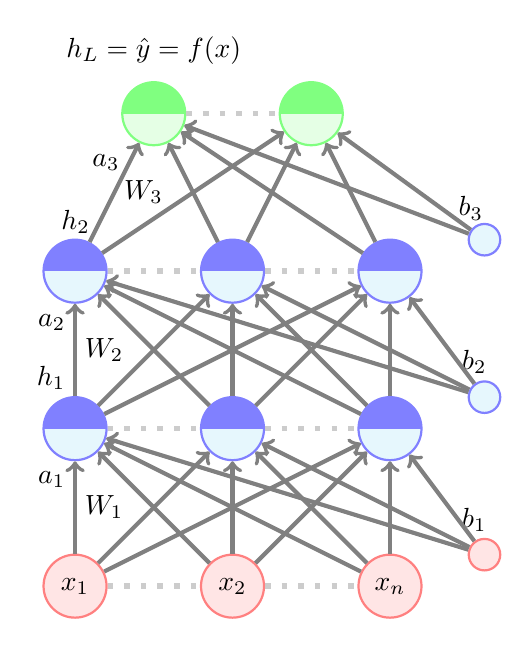
\begin{tikzpicture}
	\onslide<2->{\node [input_neuron] (neuron01) at (0,0) {$x_1$};}
	\onslide<2->{\node [input_neuron] (neuron02) at (2,0) {$x_2$};}
	\onslide<2->{\node [input_neuron] (neuron03) at (4,0) {$x_n$};}

	\onslide<13->{\node [bias_neuron] (neuron04) at (5.2,0.4) {};}


	\onslide<4->{\node [hidden_neuron] (neuron11) at (0,2)  {};}
	\onslide<4->{\node [hidden_neuron] (neuron12) at (2,2)  {};}
	\onslide<4->{\node [hidden_neuron] (neuron13) at (4,2)  {};}

	\onslide<14->{\node [bias_hidden_neuron] (neuron14) at (5.2,2.4) {};}

	\onslide<8->{
		\begin{scope}
			\path[clip] (0,2) circle (4mm);
			\path[fill=blue!50] (-0.4,2) rectangle (0.4,2.4);
		\end{scope}
		\begin{scope}
			\path[clip] (2,2) circle (4mm);
			\path[fill=blue!50] (1.6,2) rectangle (2.4,2.4);
		\end{scope}
		\begin{scope}
			\path[clip] (4,2) circle (4mm);
			\path[fill=blue!50] (3.6,2) rectangle (4.4,2.4);
		\end{scope}
	}

	\onslide<4->{\node [hidden_neuron] (neuron21) at (0,4)  {};}
	\onslide<4->{\node [hidden_neuron] (neuron22) at (2,4)  {};}
	\onslide<4->{\node [hidden_neuron] (neuron23) at (4,4)  {};}

	\onslide<15->{\node [bias_hidden_neuron] (neuron24) at (5.2,4.4) {};}

	\onslide<8->{
		\begin{scope}
			\path[clip] (0,4) circle (4mm);
			\path[fill=blue!50] (-0.4,4) rectangle (0.4,4.4);
		\end{scope}
		\begin{scope}
			\path[clip] (2,4) circle (4mm);
			\path[fill=blue!50] (1.6,4) rectangle (2.4,4.4);
		\end{scope}
		\begin{scope}
			\path[clip] (4,4) circle (4mm);
			\path[fill=blue!50] (3.6,4) rectangle (4.4,4.4);
		\end{scope}
	}

	\onslide<6->{
		\node [output_neuron] (neuron31) at (1,6)  {};
		\node [output_neuron] (neuron32) at (3,6)  {};
	}

	\onslide<8->{
		\begin{scope}
			\path[clip] (1,6) circle (4mm);
			\path[fill=green!50] (0.6,6) rectangle (1.4,6.4);
		\end{scope}
		\begin{scope}
			\path[clip] (3,6) circle (4mm);
			\path[fill=green!50] (2.6,6) rectangle (3.4,6.4);
		\end{scope}
	}

	\onslide<9->{\draw[white,->] (neuron01) -- (neuron11) node[black,pos=0.8,left] {$a_{1}$} ;}
	\onslide<9->{\draw[white,->] (neuron11) -- (neuron21) node[black,pos=0.8,left] {$a_{2}$} ;}
	\onslide<9->{\draw[white,->] (neuron21) -- (neuron31) node[black,pos=0.8,left] {$a_{3}$} ;}

	\onslide<10->{\draw[white,->] (neuron11) -- (neuron21) node[black,pos=.2,left] {$h_{1}$};}
	\onslide<10->{\draw[white,->] (neuron21) -- (neuron31) node[black,pos=.2,left] {$h_{2}$};}
	\onslide<10->{\draw[white,->] (neuron31) -- (1,6.5) node[black,pos=1,above] {$h_L = \hat{y} = f(x)$};}


	\onslide<13->{\draw[white,->] (neuron01) -- (neuron11) node[black,pos=.5,right]  {$W_{1}$} ;}
	\onslide<13->{\draw[white,->] (neuron04) -- (neuron13) node[black,pos=0,right,above] {$b_1$};}

	\onslide<14->{\draw[white,->] (neuron11) -- (neuron21) node[black,pos=.5,right] {$W_{2}$} ;}
	\onslide<14->{\draw[white,->] (neuron14) -- (neuron23) node[black,pos=0,right,above] {$b_2$};}

	\onslide<15->{\draw[white,->] (neuron21) -- (neuron31) node[black,pos=.5,right] {$W_{3}$} ;}
	\onslide<15->{\draw[white,->] (neuron24) -- (neuron32) node[black,pos=0,right,above] {$b_3$};}



	%\draw[white,->] (neuron31) -- (3,6.5) node[black,pos=1,above] {$f(x)$};
	%node[pos=1.3,above,right] {$\mathscr{L}(\theta)$};

	\onslide<2->{\draw[black!20,line width=2pt,loosely dotted] (neuron01) -- (neuron02);
		\draw[black!20,line width=2pt,loosely dotted] (neuron02) -- (neuron03);}

	\onslide<4->{\draw[black!20,line width=2pt,loosely dotted] (neuron11) -- (neuron12);
		\draw[black!20,line width=2pt,loosely dotted] (neuron12) -- (neuron13);}

	\onslide<4->{\draw[black!20,line width=2pt,loosely dotted] (neuron21) -- (neuron22);
		\draw[black!20,line width=2pt,loosely dotted] (neuron22) -- (neuron23);}

	\onslide<6->{\draw[black!20,line width=2pt,loosely dotted] (neuron31) -- (neuron32);}

	\onslide<13->{
		\foreach \from in {neuron01,neuron02,neuron03,neuron04}
		\foreach \to in {neuron11,neuron12,neuron13}
		\draw [black!50,line width=1.5pt,->] (\from) -- (\to);
	}

	\onslide<14->{
		\foreach \from in {neuron11,neuron12,neuron13,neuron14}
		\foreach \to in {neuron21,neuron22,neuron23}
		\draw [black!50,line width=1.5pt,->] (\from) -- (\to);
	}

	\onslide<15->{
		\foreach \from in {neuron21,neuron22,neuron23,neuron24}
		\foreach \to in {neuron31,neuron32}
		\draw [black!50,line width=1.5pt,->] (\from) -- (\to);
	}

\end{tikzpicture}

